\def\longueurVecteurs{1.75}
\def\angle{45}
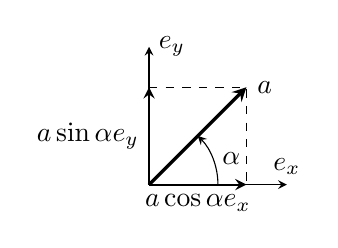
\begin{tikzpicture}
  \tikzstyle{fleche}=[->,>=stealth];
  \draw [fleche] (0,0) -- (\longueurVecteurs,0) node [above] {$\vv{e_x}$};
  \draw [fleche] (0,0) -- (0,\longueurVecteurs) node [right] {$\vv{e_y}$}; 
  \draw [fleche, very thick,\JRLblue] (0,0) -- (\angle:\longueurVecteurs) node [right] {$\vv{a}$};
  \draw [fleche] (\longueurVecteurs/2,0) arc (0:\angle:\longueurVecteurs/2) node [midway,right] {$\alpha$}; 
  \draw[fleche,thick]  (0,0)--(0:{\longueurVecteurs*cos(\angle)})node[below,midway]{$a\cos\alpha\vv{e_x}$};
   \draw[fleche,thick]  (0,0)--(90:{\longueurVecteurs*sin(\angle)})node[left,midway]{$a\sin\alpha\vv{e_y}$};
   \draw[dashed](90:{\longueurVecteurs*sin(\angle)})-|(0:{\longueurVecteurs*cos(\angle)});
\end{tikzpicture}
